\documentclass[10pt]{beamer}

\usepackage{xspace}

\newcommand{\TODO}[2][]{[\textcolor{red}{TODO (#1):} \emph{#2}]}
\newcommand{\coq}{Coq\xspace}
\newcommand{\coqdoc}{Coqdoc\xspace}
\newcommand{\coqmakefile}{\texttt{coq\_makefile}\xspace}
\newcommand{\community}{Coq-community\xspace}
\newcommand{\gaia}{Gaia\xspace}
\newcommand{\alectr}{Alectryon\xspace}
\newcommand{\equations}{Equations\xspace}
\newcommand{\Hydras}{Hydras \& Co$\text.$\xspace}
\newcommand{\make}{\texttt{make}\xspace}


\definecolor{plugincolor}{rgb}{0.6,0.0,0.6}
\definecolor{mathcolor}{rgb}{1.0,0.3,0.0}
\definecolor{coqstylecolor}{rgb}{0.0,0.0,01.0}

\definecolor{metavarcolor}{rgb}{0.5,0.0,1.0}
\definecolor{darkgreen}{rgb}{0.1,0.7,0.1}
\definecolor{answercolor}{rgb}{.08,.15,.8}
\definecolor{normalcolor}{rgb}{0.0,0.0,0.0}
\definecolor{exbluecolor}{rgb}{0.1,0.1,0.9}
\definecolor{dontlookcolor}{rgb}{0.5,0.5,0.5}
\definecolor{termcolor}{rgb}{0.0,0.1,0.9}
\definecolor{lookcolor}{rgb}{0.9,0.1,0.0}
\definecolor{prooftermcolor}{rgb}{0.3,0.1,1.0}
\definecolor{typecolor}{rgb}{1.0,0.6,0.0}
\definecolor{taccolor}{rgb}{0.70,0.10,0.0}
\definecolor{pink}{rgb}{0.8,0.6,0.6}
\definecolor{darkmagenta}{rgb}{0.4,0.0,0.6}
\definecolor{darkblue}{rgb}{0.0,0.0,0.6}


\usepackage{ifpdf}
\ifpdf
\usepackage{graphicx}
%\usepackage{aeguill}
\else
\usepackage[dvips]{graphicx}
\fi


%%%%%%%%%%%%%%%%%%%%%%%%%%%%%%%%%%%%%%%%%%%%%%%%%%%%%%%%%%%%%%
%%%% For Alectryon

\usepackage{texments}
%%% for movies by alectryon
\usepackage{./alectryon}
\usepackage{../pygments}

% Prevent breaks in the middle of syntactic units
\let\OldPY\PY
\def\PY#1#2{\OldPY{#1}{\mbox{#2}}}


%%% One hypothesis per line 
\makeatletter
\renewcommand{\alectryon@hyps@sep}{\alectryon@nl}
\makeatother

%%% \snippets{A,B,C,…} inputs a series of snippets as one block (with \itemsep
%%% between them).  A, B, C should be paths to files in snippets/.
\usepackage{etoolbox}
\makeatletter

\newcommand{\pathtomovies}{..}%/movies}

\newcommand{\inputsnippets}[1]
  {{\setlength{\itemsep}{1pt}\setlength{\parsep}{0pt}% Adjust spacing
    \alectryon@copymacros\begin{io}
      \forcsvlist{\item\@inputsnippet}{#1}
    \end{io}}}
\let\input@old\input % Save definition of \input
\newcommand{\@inputsnippet}[1]
  {{\renewenvironment{alectryon}{}{}% Skip \begin{alectryon} included in snippet
    \input@old{{\pathtomovies}/#1}}}
\makeatother

% End of Alectryon stuff
%%%%%%%%%%%%%%%%%%%%%%%%%%%%%%%%%%%%%%%%%%%%%%%%%%%%%%%%%%%
\title{Hydras \& Co.: Formalized mathematics in Coq\\
 for inspiration and entertainment
}
\date{JFLA, February 2022}
\author{
Pierre Castéran \inst{1}
\and
    Jérémy Damour \inst{2}
\and
Karl Palmskog \inst{3}
\and Clément Pit-Claudel \inst{4}
\and Théo Zimmermann \inst{5}
}

\institute{
Univ. Bordeaux, CNRS, Bordeaux INP, LaBRI, UMR 5800, F-33400 Talence, France  %\\
 % \email{pierre.casteran@labri.fr}
\and
Univ. de Paris, F-75013 Paris, France
\and
KTH Royal Institute of Technology, Stockholm, Sweden
\and
MIT CSAIL, Cambridge, Massachusetts, USA
\and
Inria, Univ. de Paris, CNRS, IRIF, UMR 8243, F-75013 Paris, France
}





\begin{document}
%%%%%%%%%%%%%%%%%%%%%%%%%%%%%%%%%%%%
\begin{frame}
  \maketitle
\end{frame}
%%%%%%%%%%%%%%%%%%%%%%%%%%%%%%%%%%%%%%
\begin{frame}
  \frametitle{Coq-community}
  \begin{block}{Objectives}
    \begin{itemize}
    \item \TODO{}{}
    \item\TODO{}{}
      \item Documentation on libraries
    \end{itemize}
  \end{block}
\end{frame}
%%%%%%%%%%%%%%%%%%%%%%%%%%%%%%%%%%%%%%%
\begin{frame}
  \frametitle{Yet another book on \coq?}
  \begin{block}{Kinds of books}
    \TODO{}{}
  \end{block}
\end{frame}
%%%%%%%%%%%%%%%%%%%%%%%%%%%%%%%%%%%%%%%%%
\begin{frame}
  \frametitle{Example-driven books (1)}
  \begin{block}{}
    \begin{itemize}
    \item \TODO{}{Definition}
    \item No need to be complete (there is already a reference manual)
      \item No need to introduce \coq (there are already a lot of initiation books and tutorials)
    \item \coq patterns (formalization and proof) are presented  when they are needed.
    \item Allow to compare several different formalizations of a given notion, and several proofs of the same theorem.
    \item By definition, the authors choose topics they like to teach.
      \item \TODO{}{topics adapted to the potential readers?}
    \end{itemize}
  \end{block}
\end{frame}
%%%%%%%%%%%%%%%%%%%%%%%%%%%%%%%%%%%%%%%%%
\begin{frame}
  \frametitle{Example-driven books (2)}
  \begin{block}{Tsukuba Coq User's Group}
    Regular languages, lambda-calculus, programming language semantics, \dots
    
   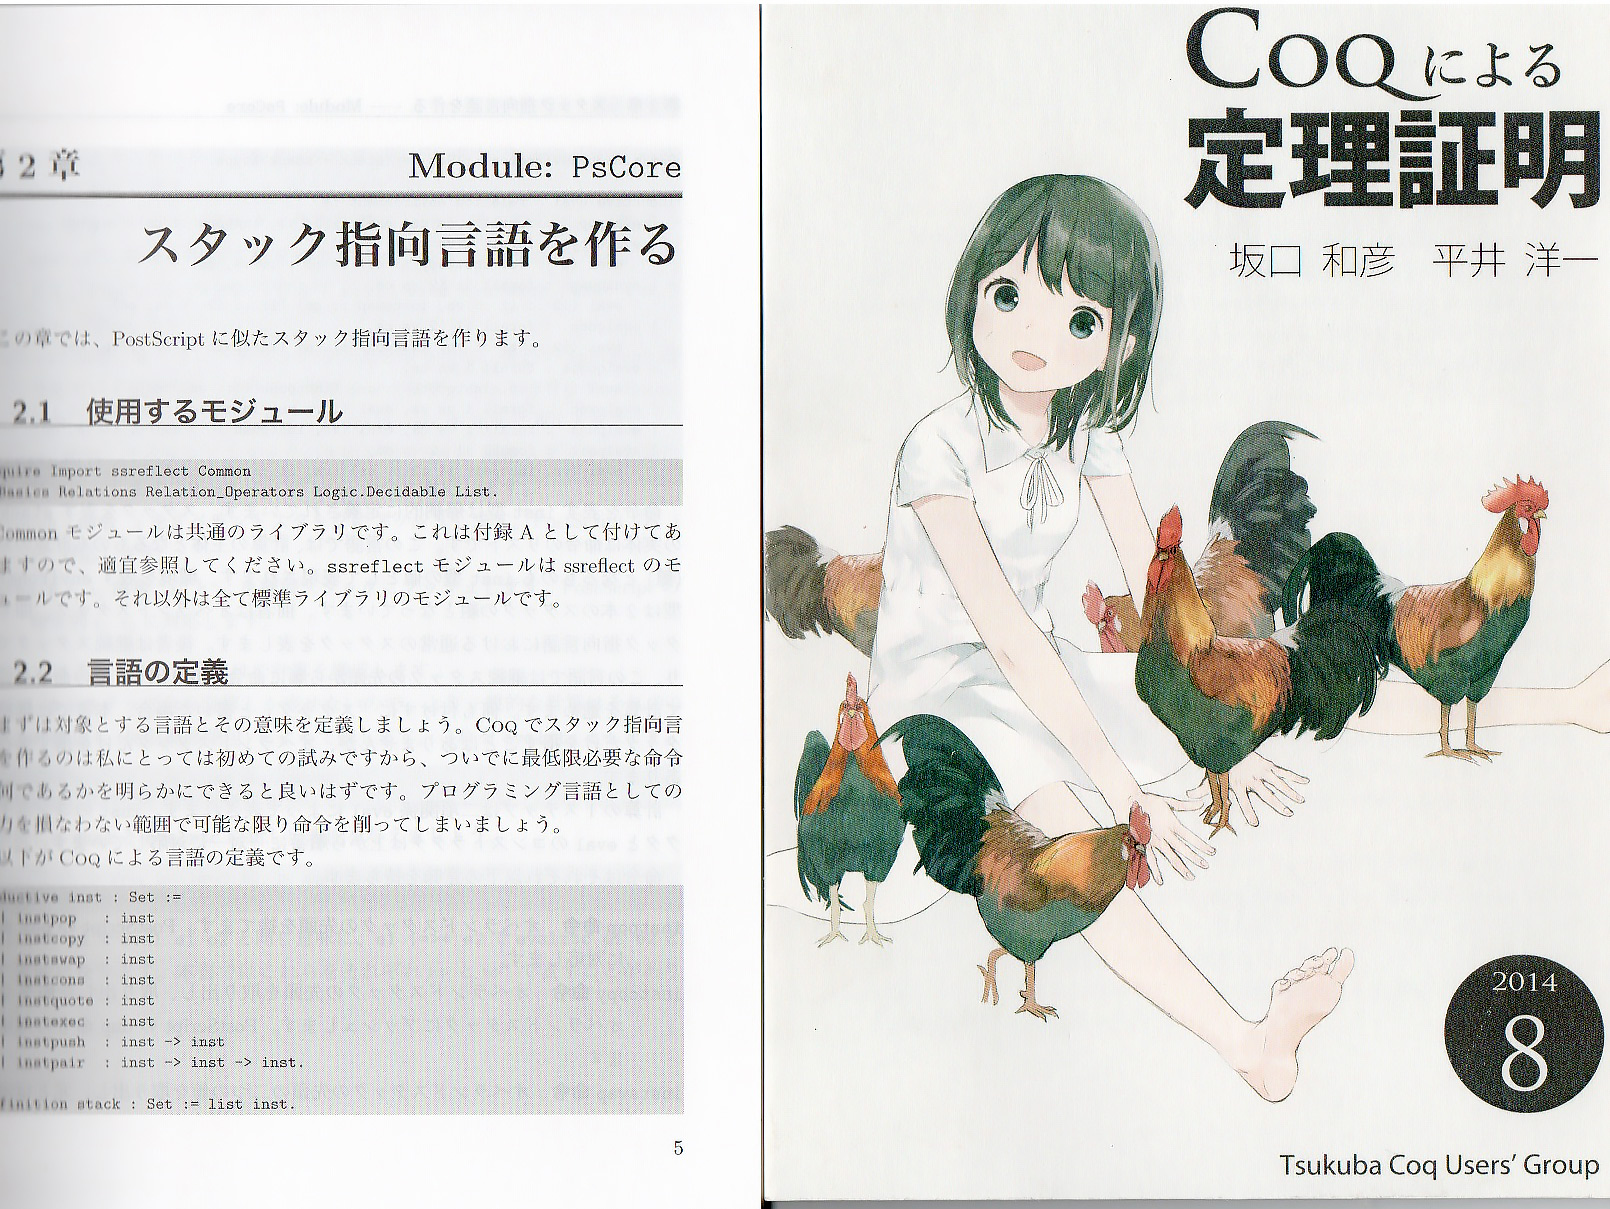
\includegraphics[height=35mm]{tsukubabooks.jpg}
   %\includegraphics[height=45mm]{leaflet.jpg}
     \end{block}
     \begin{block}{\Hydras}
       Kirby \& Paris'  hydra battles, exponentiation algorithms, \dots
     \end{block}

\end{frame}

%%%%%%%%%%%%%%%%%%%%%%%%%%%%%%%%%%%%%%
\begin{frame}
  \frametitle{What hydras are talking about?}
  \begin{block}{}
    \Hydras presents a consistent set of examples, which allow us to formalize 
    some \textcolor{mathcolor}{discrete math}, discuss
    \textcolor{coqstylecolor}{\coq style, specification and proof patterns}, and use\footnote{and depend on!} \textcolor{plugincolor}{a few plug-ins}.
  \end{block}
  \begin{block}{Hydra battles}
    \begin{itemize}
\item  \textcolor{mathcolor}{ordinals},
    \textcolor{mathcolor}{rapidly growing functions},
    \textcolor{mathcolor}{primitive recursive functions}, etc.
    \item \textcolor{coqstylecolor}{dependently typed functions},
      \textcolor{coqstylecolor}{proofs of well-foundedness},
         \textcolor{coqstylecolor}{impossibility proofs},
    \textcolor{coqstylecolor}{uniqueness of identity proofs (UIP)},
      \textcolor{coqstylecolor}{indefinite description (Hilbert's epsilon operator)},
    etc.
  \item
 \textcolor{plugincolor}{equations (Matthieu Sozeau)},
    \textcolor{plugincolor}{ackermann (Russel O'Connor)},
      \textcolor{plugincolor}{gaia (Jos\'e Grimm)}
    \end{itemize}
  \end{block}

  \begin{block}{Addition chains}
    \begin{itemize}
    \item    \textcolor{mathcolor}{algorithmics},
       \textcolor{mathcolor}{arithmetic},
  \item 
    \textcolor{coqstylecolor}{monadic notations},
    \textcolor{coqstylecolor}{PHOAS},
  \textcolor{coqstylecolor}{parametricity}, etc.
    \item
      \textcolor{plugincolor}{paramcoq (Chantal Keller, Marc Lasson)} 
          \end{itemize}
  \end{block}
\end{frame}

%%%%%%%%%%%%%%%%%%%%%%%%%%%%%%%%%%%%%%%
\begin{frame}[fragile]
  \frametitle{Tests with Alectryon(1)}
  \begin{footnotesize}
      \inputsnippets{Schutte_Ex42a}   
      \inputsnippets{Schutte_Ex42b, Schutte_Ex42c}   
    \end{footnotesize}
  \end{frame}
  %%%%%%%%%%%%%%%%%%%%%%%%%%%%%%%%%%%%%%%%
  \begin{frame}[fragile]
    \frametitle{Tests with Alectryon(2)}
      
  
  \begin{footnotesize}
  \inputsnippets{Schutte_Ex42d, Schutte_Ex42e}   
  \end{footnotesize}
 
\end{frame}
\end{document}

%%%%%%%%%%%%%%%%%%%%%%%%%%%%%%%%%%%%
\begin{frame}
  \frametitle{Introduction}
  \begin{block}{}
We show a small but non-trivial example of using Alectryon
for writing a documentation (in pdf) of a proof written in Coq.    
  \end{block}

  \begin{block}{}
    \begin{quote}
      
     `` If a   relation $<$ on a type $A$ is well founded,
    then the lexicographic exponentiation of $<$  is well-founded too.''
    \end{quote}

 \end{block}
\end{frame}


\begin{frame}[fragile]
  
  \inputsnippets{MultisetWf/tDef}

Let us consider a relation over some type $A$. We define a lexicographic order on ($\texttt{t}\;A$).

\begin{scriptsize}
\inputsnippets{MultisetWf/AGiven, MultisetWf/lexpowerDef}  
\end{scriptsize}

\begin{footnotesize}
\inputsnippets{MultisetWf/AGiven, MultisetWf/lexpowerDef}  
\end{footnotesize}

\end{frame}

\begin{frame}[fragile]
     The current goal is universally quantified over \texttt{n}.
Thus we may prove it by well founded induction over \texttt{nat}. 

\begin{small}
\inputsnippets{MultisetWf/LAccsc}
 \end{small}
\begin{footnotesize}
  \inputsnippets{MultisetWf/LAccsd}
\end{footnotesize}

  Thanks to \texttt{Hl}, we know that \texttt{l} is accessible.
Thus we can build an induction over \texttt{l}'s accessibility.

\end{frame}
\end{document}
\maketitle


Such sequences are represented in a compact way as multisets over $A$. 
For instance, $\langle a,a,a,b,c,c,c,c,c \rangle $ where $a>b>c$ is represented by the list \texttt{(a,2)::(b,0)::(c,4)::nil}.


Note that a factor $(a,n)$ is interpreted as $n+1$ copies of $a$.

\inputsnippets{MultisetWf/tDef}

Let us consider a relation over some type $A$. We define a lexicographic order on ($\texttt{t}\;A$).

\inputsnippets{MultisetWf/AGiven, MultisetWf/lexpowerDef}

\section{\texttt{lexpower}  is not well-founded in general}

Let us build an infinite strictly decreasing (w.r.t. \texttt{lexpower lt}) sequence.


\inputsnippets{MultisetWf/notWfa}

Then, we prove that any element of the sequence \texttt{seq} is non-accessible.

\inputsnippets{MultisetWf/notWfb}

It's clearly a contradiction, since (\texttt{seq 0}) is an element of the sequence, and accessible (because of the hypothesis \texttt{Hwf}).

\inputsnippets{MultisetWf/notWfc}
\section{Lists in normal form}


We say that a list $(a_1,n_1)::(a_2,n_2)::\dots::(a_p,n_p)::nil$  in  (\texttt{t A}) is in \emph{normal form} if  for any $1<=i<n$,
we have $\texttt{ltA}\; a_{i+1}\; a_i$.

\inputsnippets{MultisetWf/lexnfDef}

The \emph{lexicographic exponentiation} of \texttt{ltA} is the restriction
of \texttt{lexpower ltA} to the set of lists in normal form.
In the next section, we prove that, if \texttt{ltA} is well-founded, then its lexicographic power is well-founded too.
\inputsnippets{MultisetWf/lexltDef}

\paragraph{Note:} The restriction of a binary relation to a set is defined in the file \texttt{Restriction.v}.

\inputsnippets{Restriction/restrictionDef}


\section{Proof of well-foundedness}
It's time to prove that the lexicographic power of a well-founded relation is well-founded too. Let us open a work section.

\inputsnippets{MultisetWf/bigProofa}

We want to prove the following statement:

\inputsnippets{MultisetWf/theStatement}



\subsection{A first attempt}
We may try to prove \texttt{lexwf} by (structural) induction on \texttt{l}.

\inputsnippets{MultisetWf/BadProof,
  MultisetWf/BadProofb}

By the hypothesis \texttt{H0}, the list \texttt{y} may be
equal to \texttt{(a,n)::l'}, where \texttt{LT l' l}. But the induction hypothesis \texttt{IHl} is useless for solving the current goal.
\inputsnippets{MultisetWf/BadProofc}

This is a classical issue. In a naive proof by induction, some variables are fixed too early: here, the variable \texttt{l} in \texttt{IHl}.

\subsection{Introducing a new predicate}

We can express the well-foundedness of \texttt{LT} in the following way :
\begin{quote}
  \begin{enumerate}
    \item  ``The empty list is accessible''
  \item   `` For any $a$ in $A$ and $n$ in \texttt{nat},  any well-formed list starting with $(a,n)$ is accessible. ''

  \end{enumerate}
 \end{quote}

The first property is easy to prove by inversion.
 
\inputsnippets{MultisetWf/AccNil}

For the second one, we define a new predicate over $A$.
 
\inputsnippets{MultisetWf/AccsDef}

The new goal is to prove that any element of $A$ satisfies
the predicate \texttt{Accs}.


\subsection{Inversion lemmas}

Before starting the proof, we  prove three useful inversion lemmas:

\inputsnippets{MultisetWf/NFInv1}
\inputsnippets{MultisetWf/NFInv2}
\inputsnippets{MultisetWf/LTInv}

\subsection{The proof by induction}
Le us prove, by induction on $a:A$ that every element of $A$ satisfies \texttt{Accs}.

\inputsnippets{MultisetWf/LAccsa}

Let us note that, for any list \texttt{(a,n)::l} in normal form,
the tail \texttt{l} is either empty or starts with some pair \texttt{(b,p)} where \texttt{ltA b a}, hence is accessible (thanks to \texttt{IHa}).

\inputsnippets{MultisetWf/LAccsb}
\inputsnippets{MultisetWf/LAccsg}

The current goal is universally quantified over \texttt{n}.
Thus we may prove it by well founded induction over \texttt{nat}. 

\inputsnippets{MultisetWf/LAccsc, MultisetWf/LAccsd}

Thanks to \texttt{Hl}, we know that \texttt{l} is accessible.
Thus we can build an induction over \texttt{l}'s accessibility.




\inputsnippets{MultisetWf/LAccse}

In order to prove the accessibility of the list \texttt{((a, n) :: x0)}, we have to prove that any predecessor $y$ of this list is accessible, and consider every case (thanks to \texttt{LT\_inv}).

\inputsnippets{MultisetWf/LAccsf}

\subsubsection{First case}
If \texttt{y=nil}, then \texttt{y} is clearly accessible. 


\inputsnippets{MultisetWf/case1}

\subsubsection{Second case}
Let us consider a well formed list \texttt{y} of the form \texttt{(b,p)::l''}, where \texttt{ltA b a}. By \texttt{IHa}, this list is accessible.

\inputsnippets{MultisetWf/case2}

\subsubsection{Third case}
The list \texttt{y} may be of the form  \texttt{(a,n)::l''}, where \texttt{LT l'' l}. By \texttt{H2},  \texttt{y} is accessible.

\inputsnippets{MultisetWf/case3}
  
\subsubsection{Last case}
The list \texttt{y} may be of the form  \texttt{(a,p)::l''}, where \texttt{p<n}. Thus, we may apply \texttt{Hn}.


\inputsnippets{MultisetWf/case4}

\subsection{At last!}


\inputsnippets{MultisetWf/NFAcc}


\inputsnippets{MultisetWf/lexwf}




% \section{Examples}

% \inputsnippets{MultisetWf/Examples}

\section{Impossibility proofs}
There is no function of type \texttt{t nat ->  nat} which could serve as a measure for proving \texttt{lexlt lt}'s well-foundedness.


\inputsnippets{MultisetWf/Impossibility1}
\inputsnippets{MultisetWf/Impossibility1a}
\inputsnippets{MultisetWf/Impossibility1b}

\emph{Same exercise with \texttt{nat*nat} (with the lexicographic square of \texttt{lt})}.

\end{document}
